%-------------------------------------------------------------------------------
%-------------------------------------------------------------------------------
%-------------------------------------------------------------------------------
\chapter{Équations différentielles}
%-------------------------------------------------------------------------------
%-------------------------------------------------------------------------------
\thispagestyle{empty}
%-------------------------------------------------------------------------------
%-------------------------------------------------------------------------------
{\sf Depuis Newton les lois de la physique sont souvent écrites sous formes d'équations reliant des fonctions à déterminer et leurs dérivées. 

Nous allons, dans ce chapitre, préciser les notions d'équations différentielles générales et de solutions, particulièrement de solution approchée et donner un algorithme simple qui permet de déterminer des solutions approchées.

Le but sera de résoudre de manière approchée la plupart des équations, pas de résoudre mathématiquement un petit nombre d'équations.
}
%-------------------------------------------------------------------------------
%--------------------------------------------------------------------------
\section{Présentation}
%--------------------------------------------------------------------------
%--------------------------------------------------------------------------
%--------------------------------------------------------------------------
\subsection{Introduction}
%--------------------------------------------------------------------------


{\bf On appelle équation différentielle  une relation entre une ou plusieurs fonctions inconnues et leurs dérivées.} 

L'{\it ordre} d'une équation différentielle correspond au degré maximal de dérivation auquel l'une des fonctions inconnues a été soumise. 

Voici quelques exemples.
%--------------------------------------------------------------------------
\begin{description}
%--------------------------------------------------------------------------
\item[Radioactivité] On note $N(t)$ le nombre de noyaux radioactifs à l'instant $t$, c'est-à-dire se désintégrant selon un processus aléatoire. 

Il existe un nombre $\lambda$ dit {\it  constante radioactive} tel que $N'(t)=-\lambda N(t)$.

L'ordre est ici 1. On peut écrire $N'(t) = f\bigl((t,N(t)\bigr)$ avec $f$ : $(t,u)\mapsto -\lambda u$.
%--------------------------------------------------------------------------
\item[Oscillations libres] Un ressort exerce une force opposée et proportionnelle à l'allongement du ressort $F = -kx$.

Si on néglige les frottements, l'équation $m\vec{a} =\sum\vec{ F} $ donne $mx'' = -kx$.

En notant $\omega_0=\sqrt{\frac{k}{m}}$ on peut aussi écrire l'équation sous la forme $x'' +\omega_0^2x=0$ : c'est une équation d'ordre 2.
%--------------------------------------------------------------------------
\item[Pendule] L'équation du pendule pesant peut s'écrire $\displaystyle \theta'' =\frac gl\sin(\theta)$ où $\theta$ est l'angle avec la verticale et $l$ est la longueur. C'est une équation d'ordre 2 et elle n'est pas linéaire : l'expression n'est pas linéaire en la fonction inconnue et ses dérivées.

\end{description}
%--------------------------------------------------------------------------
Nous allons nous restreindre dans ce chapitre au cas des équations d'ordre 1. \footnote{Nous verrons que cette limite est surmontable.} et résolues en $y'$.

\newpage
%--------------------------------------------------------------------------
\subsection{Définitions}
%--------------------------------------------------------------------------
Nous traitons donc des équations de la forme
\[y' = \varphi(y,t)\leqno(E)\]

où $\varphi$ est définie et continue sur une partie de $\R^2$ de la forme $U=]a;b[\times ]c;d[$\footnote{Plus généralement sur un ouvert de $\R^2$.} et à valeur dans $\R$.

\medskip

Une {\bf solution} de $(E)$ est la donnée d'un intervalle $I$ de $\R$ et d'une fonction $f$ de classe ${\cal C}^1$ sur $I$  tels que 
%--------------------------------------------------------------------------
\begin{itemize}
  \item $\bigl(t,\varphi(t)\bigr)\in {\cal U}$ pour tout $t\in I$,
  \item $f'(t)= \varphi\bigl(f(t),t \bigr)$ pour tout $t\in I$.
\end{itemize}
%--------------------------------------------------------------------------
Géométriquement cela signifie qu'une solution est telle que sa tangente en un point $\bigl(t,f(t)\bigr)$ admet $ \varphi\bigl(f(t),t \bigr)$ pour pente.

\def\k{-0.25}
%--------------------------------------------------------------------------
\begin{center}
\tikzpicture [scale=0.8] 
\draw[-stealth] (-6,0)--(6,0) node [below] {$t$}; 
\draw[-latex] (0,0)--(1,0); 
\draw[-stealth] (0,-3)--(0,3) node [left] {$y$}; 
\draw[-latex] (0,0)--(0,1); 
\foreach \a in {-5.5,-5,...,5.5}
 \foreach \b in {-2.5,-2,...,2.5}
 \draw[->] (\a,\b)--+(0.2,{0.2*(((3*\a*\a+1)*\k-2*\a*\b)/(\a*\a+1)});
\foreach \c in {-2,0,1,3}
 \draw [samples=100,domain=-5.5:5.5] plot(\x,{\c/(\x*\x+1)+\x*\k});
\endtikzpicture 
\end{center}
%--------------------------------------------------------------------------
\medskip

Une équation aura beaucoup de solutions possibles. On spécialise l'équation $(E)$ en ajoutant des {\bf conditions initiales}, c'est un couple $(t_0,y_0)\in U$ et on cherche une solution passant par ce point : une solution doit vérifier $f(t_0) = y_0$. On obtient un {\bf problème de Cauchy} :
\[\left\{\begin{matrix} y' = \varphi(y,t)\\ y(t_0)=y_0\end{matrix}\right.\leqno(E_0)\]


Si $\varphi$ est suffisamment régulière, le théorème de Cauchy-Lipschitz affirme l'existence d'un intervalle ouvert $I$ contenant $t_0$ et d'une unique fonction $f$ de classe ${\cal C}^1$ sur $I$ tels que $(I,f)$ est une solution de $(E_0)$.

\medskip

Le problème que nous chercherons à résoudre sera de déterminer une approximation de la solution sur un intervalle $[t_0,t_f]$ (ou $[t_f;t_0]$) avec les conditions initiales $(t_0,y_0)$. On admettra qu'une telle solution existe : en particulier nous supposerons que $\varphi$ vérifie les conditions de régularité.
%--------------------------------------------------------------------------
\subsection{Vers la résolution}
%--------------------------------------------------------------------------
Que veut-on calculer ?

On a déjà vu une équation différentielle particulière : calculer l'intégrale $\displaystyle \int_a^b g(t)\d t$ revient à calculer la valeur en $b$ de la solution de 
\[\left\{\begin{matrix} y' = f(t)\\ y(a)=0\end{matrix}\right.\leqno(E_{int})\]

En effet, les solutions de $y' = f(t)$ sont les primitives de $f$, et si on choisit la primitive $F$ de $f$ qui s'annule en $a$, on a $\displaystyle \int_a^b g(t)\d t = F(b)$.

Lors du calcul de l'intégrale on n'a renvoyé que cette valeur mais lors du calcul, on a calculé un grand nombre de valeurs intermédiaires qui permettent en fait de calculer les valeurs approchées de $\displaystyle \int_a^{a_k} f(t)\d t$ avec $\displaystyle a_k = a + k\frac{b-a}n$.

Si on garde ces valeurs dans une liste, on obtient une liste de valeurs approchées des $F(a_k)$.

Voici une possibilité avec la méthode des trapèzes.
%--------------------------------------------------------------------------
\begin{lstlisting}[caption=Valeurs d'une primitive]
def primitive(f, a, b, n):
    """Entree : une fonction f,
                deux bornes,
                un entier
       Sortie : deux listes,
                la première contient les points de la subdivision,
                la seconde, les valeurs de la primitive en ces points"""
    pas = (b-a)/n
    T = [0]*(n+1)        # liste des points de subdivision
    F = [0]*(n+1)        # liste des valeurs de la primitive
    T[0] = a             # initialisation
    F[0] = 0             # initialisation
    for k in range(n):   # il reste n valeurs
        T[k+1] = a + (k+1)*(pas
        F[k+1] = F[k] + pas*(f(T[k]) + f(T[k+1]))/2
    return T, F
\end{lstlisting}
%--------------------------------------------------------------------------
\medskip

On va garder ce même principe mais, au lieu de donner les paramètres $a$, $b$ et $n$, nous allons utiliser comme paramètre la liste des points en lesquels on veut une valeur approchée de la solution. Les méthodes renverront simplement la liste des valeurs en ces points.

%--------------------------------------------------------------------------
\begin{enumerate}
  \item On définit une liste \type{T} de taille $n$ avec $t_0=\type{T[0]} $ et $t_f=\type{T[n-1]}$
  \item On cherche une liste \type{Y} de taille $n$ aussi telle que \type{Y[k]} est une valeur approchée de $f\bigl(\type{T[k]}\bigr)$
\end{enumerate}
%--------------------------------------------------------------------------
{\bf Remarques}
%--------------------------------------------------------------------------
\begin{enumerate}
\item Le plus souvent la suite des valeurs de \type{T} sera régulièrement espacée mais ce ne sera pas imposé.
%--------------------------------------------------------------------------
\item Les suites \type{T} et \type{Y} permettent de visualiser le graphe de la solution. 
%--------------------------------------------------------------------------
\begin{lstlisting}
plt.plot(T, Y)
plt.show()
\end{lstlisting}
%--------------------------------------------------------------------------
La représentation trace les segments délimités par les points de coordonnées \type{(T[k], Y[k])}.
\end{enumerate}
%--------------------------------------------------------------------------
%--------------------------------------------------------------------------
\section{Quelques méthodes}
%--------------------------------------------------------------------------
%--------------------------------------------------------------------------
On va écrire des fonctions de résolution de la forme
%--------------------------------------------------------------------------
\begin{lstlisting}
def solution(phi, y0, T):
    ...
    return Y
\end{lstlisting}
%--------------------------------------------------------------------------
On rappelle que l'on cherche à approcher la solution de 
\[\left\{\begin{matrix} y' = \varphi(y,t)\\ y(t_0)=y_0\end{matrix}\right.\leqno(E_0)\]
sur un intervalle $[t_0; t_f]$ ou $[t_f; t_0]$.
%--------------------------------------------------------------------------
\subsection{Paramètres utilisés}
%--------------------------------------------------------------------------
\begin{description}
\item[\type{phi} : fonction de l'équation] On doit donner la fonction qui définit l'équation différentielle.

Exemple : l'équation $\tau y'(t)+y(t)=Ke_0$ soit : $y'(t)=\frac{Ke_0-y(t)}{\tau}$ pourra s'écrire
%--------------------------------------------------------------------------
\begin{lstlisting}
def phi(y,t):
    K = 2.5
    e0 = 1.7
    tau = 0.25
    return (y - K*e0)/tau
\end{lstlisting}
%--------------------------------------------------------------------------
On remarquera que les variables sont \type{y} suivie de \type{t}; c'est la convention prise dans les modules qu'on utilisera parfois, en particulier \type{scipy.integrate}.

Il arrivera très souvent dans les équations qui seront utilisées que la variable $t$ n'apparaisse pas explicitement dans $\varphi$, comme ici. Il faudra néanmoins introduire $t$ comme paramètre.
%--------------------------------------------------------------------------
\item[\type{y0} : condition initiale] La valeur de $t_0$ est donnée par la première valeur de \type{T}. Il reste donc à donner la valeur initiale du problème de Cauchy : $y_0$.
%--------------------------------------------------------------------------
\item[\type{T} : liste des temps] L'intervalle de temps est discrétisé en une suite finie de temps. On notera $t_k$ la valeur de \type{T[k]}. Le plus souvent les valeurs de la liste seront séparées par un pas constant : $t_k = t_0 + k\frac{t_f - t_0}{n-1}=t_0+k(t_1-t_0)$ si $n$ est la longueur de \type{T}.
%--------------------------------------------------------------------------
\item[\type{Y} : résultat] C'est la liste des valeurs approchées des $f(t_k)$. On note $y_k = \type{Y[k]}$.
\end{description}
%--------------------------------------------------------------------------
\subsection{Principe}
%--------------------------------------------------------------------------
Pour définir la suite $Y$ à  partie de $T$, $y_0$ et $\varphi$ nous allons procéder pas-à-pas.
%--------------------------------------------------------------------------
\begin{enumerate}
  \item On remplace l'équation différentielle par une équation intégrale 
  
$\displaystyle f(t_{k+1})= f(t_k) + \int_{t_k}^{t_{k+1}} f'(t) \d t= f(t_k) + \int_{t_k}^{t_{k+1}}  \varphi\bigl(f(t),t \bigr) \d t$.
%--------------------------------------------------------------------------
\item On calcule, pour chaque intégrale, une valeur approchée
$\displaystyle \int_{t_k}^{t_{k+1}}  \varphi\bigl(f(t),t \bigr) d t \simeq \delta_k$.
%--------------------------------------------------------------------------
\item On définit  $y_{k+1}=y_k+\delta_k$ pour $0\le k < N$.
\end{enumerate}
%--------------------------------------------------------------------------
Les différentes méthodes correspondent à différents algorithmes d'approximation d'une intégrale.
%--------------------------------------------------------------------------
%--------------------------------------------------------------------------
\subsection{Méthode d'Euler explicite}
%--------------------------------------------------------------------------
%--------------------------------------------------------------------------
Elle correspond à la méthode des rectangles à gauche.

%--------------------------------------------------------------------------
\[ \int_{t_k}^{t_{k+1}}  \varphi\bigl(f(t),t \bigr) \d t\simeq 
(t_{k+1} - t_k) \varphi\bigl(f(t_k), t_k \bigr)\]
%--------------------------------------------------------------------------
On connaît une valeur approchée de $f(T_k)$, c'est $y_k$. Ainsi on aboutit à 
%--------------------------------------------------------------------------
\[y_{k+1}= y_k + (t_{k+1} - t_k) \varphi\bigl(y_k,t_k \bigr)\]
%--------------------------------------------------------------------------
\begin{center}
\tikzpicture [scale=1.1] 
\draw[-stealth] (-1,0)--(6,0) node [below] {$t$}; 
\draw[-latex] (0,0)--(1,0); 
\draw[-stealth] (0,-2)--(0,4) node [left] {$y$}; 
\draw[-latex] (0,0)--(0,1); 
\draw [samples=100,domain=-0.5:5.5] plot(\x,{-0.1*(\x-2)*(\x-4)+0.4*\x+0.7});
\draw (2,0) node[below]{$t_{k}$} -- (2,1.5) -- (2,1.7);
\draw[dotted] (0,1.5) node[left]{$f(t_{k})$} -- (2,1.5);
\draw[dotted] (0,1.7) node[above left]{$y_k$} -- (2,1.7) -- (6,1.7);
\draw (4,0) node[below]{$t_{k+1}$} -- (4,2.3) -- (4,2.95);
\draw[dotted] (0,2.3) node[left]{$f(t_{k+1})$} -- (4,2.3);
\draw[dotted] (0,2.95) node[above left]{$y_{k+1}$} -- (4,2.95) -- (6,2.95);
\draw[thick] (2,1.7) -- (4,2.95);
\draw[<->] (2,1) -- node[below]{$h$} (4,1);
\draw[<->] (6,1.7) --node[right]{$h\varphi\bigl(y_k,t_k \bigr)$} (6,2.95);
\draw [samples=100,domain=1.5:4.5,dashed] plot(\x,{-0.08*(\x-2)*(\x-4)+0.5*\x+0.7});
\endtikzpicture 
\end{center}
%--------------------------------------------------------------------------
On peut remarquer que $t \mapsto y_k + (t - t_k) \varphi\bigl(y_k,t_k \bigr)$ est l'équation de la tangente en $(t_k,y_k)$ de la solution de condition initiales $t_k$ et $y_k$. 

La méthode revient à suivre la tangente des solutions sur des intervalles $[t_k;t_{k+1}]$. 

On approche donc  la solution par une fonction  affine sur chaque intervalle.
%--------------------------------------------------------------------------
\begin{center}
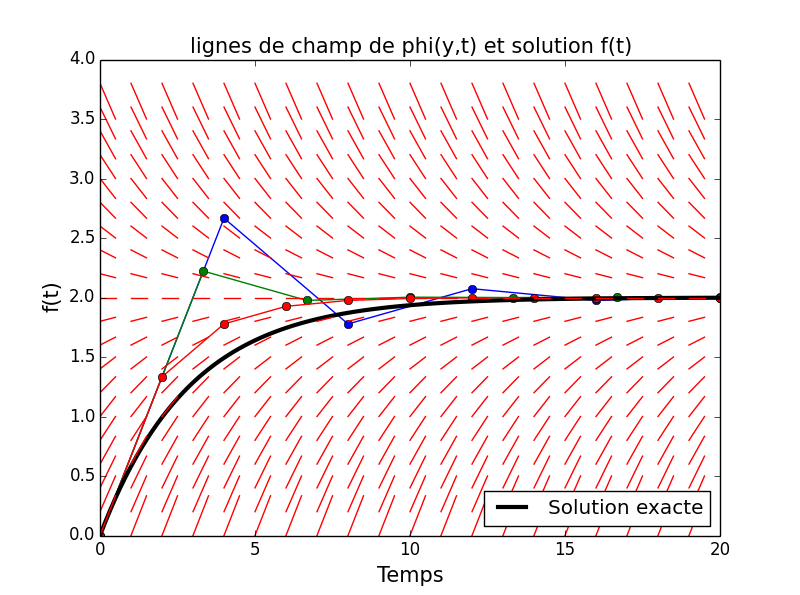
\includegraphics[width=0.9\linewidth]{14_trace-ordre1-champ.png}
\end{center}
%--------------------------------------------------------------------------
\newpage
%--------------------------------------------------------------------------
\begin{lstlisting}[numbers=left, caption=Euler explicite]
def euler(f, y0, T):
    """Entree : une fonction f de 2 variables
                un reel y0, la condition initiale en t0
                une liste de réels, monotone, dont le premier terme est t0
       Sortie : une liste de  points définissant 
                  une solution approchee de y' = f(y, t)
                  avec les conditions initiales (t0,y0)
                  y(T[i]) est approché par Y[i]"""
    n = len(T)           # n valeurs à calculer
    Y = [0]*n            # création de la liste
    Y[0] = y0            # ordonnee initiale
    for k in range(n-1): # il reste (n-1) points à trouver
        pas = T[k+1] - T[k]
        pente = f(Y[k],T[k])
        Y[k+1] = Y[k] + pas*pente # On applique la formule
    return Y
\end{lstlisting}
%--------------------------------------------------------------------------

On notera qu'on calcule le pas à chaque étape : il n'est peut-être pas constant.
%--------------------------------------------------------------------------
\subsection{Méthode d'Euler implicite}
%--------------------------------------------------------------------------
Si on approche la fonction à intégrer, $\varphi\bigl(f(u),u\bigr)$, par sa valeur finale sur l'intervalle $[t_k;t_{k+1}]$ c'est-à-dire $\varphi\bigl(f(u),u\bigr) \simeq \varphi\bigl(f(t_{k+1}),t_{k+1}\bigr)\simeq \varphi \bigl(y_{k+1},y_{k+1}\bigr)$ on obtient
%--------------------------------------------------------------------------
\[y_{k+1} =  y_k+\int_{y_{k}}^{y_{k+1}}\varphi \bigl(y_{k+1},y_{k+1}\bigr) \d t  \simeq y_k+ (t_{k+1}-t_k) \varphi \bigl(y_{k+1},t_{k+1}\bigr)\]
%--------------------------------------------------------------------------
On voit que $y_{k+1}$ apparaît aussi dans le second membre : il est défini implicitement c'est-à-dire qu'on ne peut pas le calculer directement.

Pour déterminer $y_{k+1}$ en fonction de $y_k$ il faut donc résoudre, à chaque étape, 
l'équation $g_k(y)=0$ avec $g_k(y)= y-y_k - (t_{k+1}-t_k) \varphi(y, t_{k+1})$. 

On peut, par exemple, en déterminer une valeur approchée avec des méthodes d'analyse numérique comme celle de Newton.

\medskip 

Parfois on peut résoudre directement l'équation. Par exemple si on veut résoudre l'équation différentielle $y'=y^2+t^2$ pour $y(t_0)=y_0$ sur $[t_0;t_1]$ par la méthode d'Euler implicite, on doit doit calculer les $y_k$ avec  $y_{k+1} = y_k + h \bigl(y_{k+1}^2+t_{k+1}^2\bigr)$ où $h$ est le pas supposé constant.

Ainsi $y_{k+1}$ est solution de $h X^2-X+\bigl(y_k+ht_{k+1}^2\bigr)=0$.

Les racines sont $\displaystyle \frac{1\pm\sqrt{1-4hy_k-4h^2t_{k+1}^2}}{2h}$ ; on choisit celle qui est proche de $y_k$ 
\[Y_{k+1} = \frac{1 - \sqrt{1-4hy_k-4h^2t_{k+1}^2}}{2h}\]
%--------------------------------------------------------------------------
\begin{lstlisting}
def solution_particuliere(y0, T):
    n = len(T)
    Y = [0]*n 
    Y[0] = y0
    for k in range(n-1): 
        pas = T[k+1] - T[k]
        delta = 1 - 4*pas*(Y[k]+pas*T[k+1]**2)
        Y[k+1] = (1-delta**(1/2))/(2*h)
    return Y
\end{lstlisting}
%--------------------------------------------------------------------------
\medskip

Sans rentrer dans la théorie, on peut retenir que la méthode  implicite est souvent moins précise et  plus compliquée à utiliser mais elle est  plus stable  que la méthode  explicite, elle diverge moins rapidement.
Pour simplifier grossièrement  : la méthode implicite est moins précise à court terme mais plus précise à long terme.
%--------------------------------------------------------------------------
%--------------------------------------------------------------------------
\subsubsection{Utilisation de la méthode de Newton.}
%--------------------------------------------------------------------------
On rappelle la méthode de Newton
%--------------------------------------------------------------------------
\begin{lstlisting}
def newton(f, df, x0, epsilon = 1e-8):
    h = 1 + epsilon
    x = x0
    while h > epsilon:
        x_old = x
        x = x - f(x)/df(x)
        h = abs(x - x_old)
    return x    
\end{lstlisting}
%--------------------------------------------------------------------------
L'équation à résoudre est $f(y) = y-y_k - (t_{k+1}-t_k) \varphi(y, t_{k+1})=0$.

On a $\displaystyle f'(y) = 1 - (t_{k+1}-t_k) \frac{\partial \varphi(y, t_{k+1})}{\partial y}$ : il faudra donc définir aussi la fonction python associée à la dérivée partielle.

Par exemple pour $\displaystyle y' = \frac{\sin(y)}{t^2+0.0001}$ on écrit

\medskip
%--------------------------------------------------------------------------
\begin{lstlisting}
def phi(y, t):
    return -sin(y)/(t**2+0.001)

def dphi(y, t):
    return -cos(y)/(t**2+0.001)
\end{lstlisting}
%--------------------------------------------------------------------------
La fonction a été choisie pour mettre en évidence l'amélioration de la stabilité par la méthode implicite. La solution attendue est celle fournie par la méthode implicite.

\medskip


Les fonctions $g$ et $g'$ dépendent des valeurs calculées $t_{k+1}$ et $y_k$ : on les définira à l'intérieur de la fonction de résolution, cela est possible dans python.

On prendra $y_k$ pour valeur initiale de la recherche, c'est une valeur proche de $y_{k+1}$.
%--------------------------------------------------------------------------
\begin{lstlisting}[numbers=left, caption=Euler implicite]
def euler_imp(phi, dphi, y0, T):
    n = len(T)   
    Y = [0]*n            
    Y[0] = y0           
    for k in range(N-1):  
        pas = T[k+1] - T[k]
        def f(y):
            return y - Y[i] - pas*phi(y, T[k+1])
        def df(y):
            return 1 - pas*dphi(y, T[k+1])
        Y[k+1] = newton(f, df, Y[k])
    return Y
\end{lstlisting}
%--------------------------------------------------------------------------
%--------------------------------------------------------------------------
\begin{center}
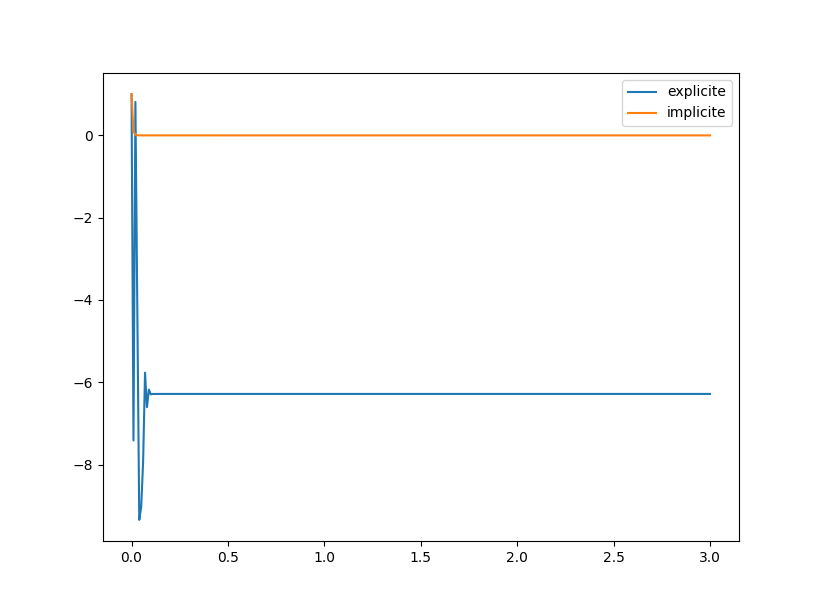
\includegraphics[width=0.9\linewidth]{14_exp_imp.png}
\end{center}
%--------------------------------------------------------------------------
%--------------------------------------------------------------------------
\subsection{Utilisations du module \type{scipy}}
%--------------------------------------------------------------------------
%--------------------------------------------------------------------------
\subsection{odeint}
%--------------------------------------------------------------------------
Le module \type{scipy} contient, dans la sous-bibliothèque \type{integrate} une fonction \type{odeint} qui résout efficacement les équations différentielles. C'est la méthode à utiliser quand la résolution d'une équation est un outil d'un projet plus large.
%--------------------------------------------------------------------------
\begin{lstlisting}
from scipy.integrate import odeint

odeint(phi,y0,T)
\end{lstlisting}
%--------------------------------------------------------------------------
\subsection{fsolve}
%--------------------------------------------------------------------------
Dans le cas de la méthode d'Euler implicite la résolution de l'équation implicite peut se faire avec la fonction \type{fsolve} (voir {\bf \ref{chap:zero}.\ref{sec:fsolve}}). 

L'usage des paramètres envoyés permet de ne définir qu'une seule fois une fonction.
%--------------------------------------------------------------------------
\begin{lstlisting}[numbers=left, caption=Euler implicite avec \type{fsolve}]
from scipy.optimize import fsolve

def euler_imp(phi, y0, T):
    def equ(y, y_old, t):
        return y - y_old - pas*phi(y_old, t)
    n = len(T)   
    Y = [0]*n            
    Y[0] = y0 
    for k in range(N-1):  
        pas = T[k+1] - T[k]
        Y[k+1] = fsolve(equ, Y[k], args = (Y[k], T[k+1]))
    return Y
\end{lstlisting}
%--------------------------------------------------------------------------
%--------------------------------------------------------------------------
%--------------------------------------------------------------------------
